%%%%%%%%%%%%%%%%%%%%%%%%%%%%%%%%%%%%%%%%%%%%%%%%%%%%%%%%%%%%%%%%%%%%%%%%%%%%%%%

\section*{\large Exercício 3}
\addcontentsline{toc}{chapter}{\protect\numberline{}\large Exercício 3}%

% EXEMPLO PARA ADICIONAR FIGURA
%\begin{figure}[ht!]
	%\caption{Série e histogramas.}
%	\vspace{0mm}	% acrescentar o espaçamento vertical apropriado entre o título e a borda superior da figura
%	\begin{center}
%		\resizebox{15cm}{!}{\includegraphics{Figuras/ex1/Exercicio1_n_64.jpg}}		
%	\end{center}
%	\vspace{-2mm}	% acrescentar o espaçamento vertical apropriado entre a borda inferior da figura e a legenda ou a fonte quando não há legenda (o valor pode ser negativo para subir)
%	\legenda{Figura 1.1: Dez sinais e seus respectivos histogramas para  asérie com $N$ = 64 do grupo noise.}	% legenda - para deixar sem legenda usar comando \legenda{} (nunca deve-se comentar o comando \legenda)
%	\label{ex1_fig1}
%	%\FONTE{}	% fonte consultada (elemento obrigatório, mesmo que seja produção do próprio autor)
%\end{figure}

%====================================================================== 3.1

\subsection*{3.1} 
\addcontentsline{toc}{section}{\protect\numberline{} 3.1}%

As Figuras 3.1 e 3.2 a seguir ilustram as propriedades de \textit{time scaling} e \textit{frequency scaling}:

\begin{align*}
f(at) &\Leftrightarrow  \frac{1}{|a|}\hat{f}\left( \frac{\xi}{a} \right) \tag*{\textit{time scaling}} \\
\frac{1}{|a|} f \left( \frac{t}{a} \right) &\Leftrightarrow \hat{f}(a \xi) \tag*{\textit{frequency scaling}} \\
\end{align*}

% EXEMPLO PARA ADICIONAR FIGURA
\begin{figure}[ht!]
	\legenda{Figura 3.1: Exemplo de \textit{time scaling} e \textit{frequency scaling} sobre a função $f_{1}(t)=e^{-|t|}$.}
	\vspace{-1mm}	% acrescentar o espaçamento vertical apropriado entre o título e a borda superior da figura
	\begin{center}
		\resizebox{\textwidth}{!}{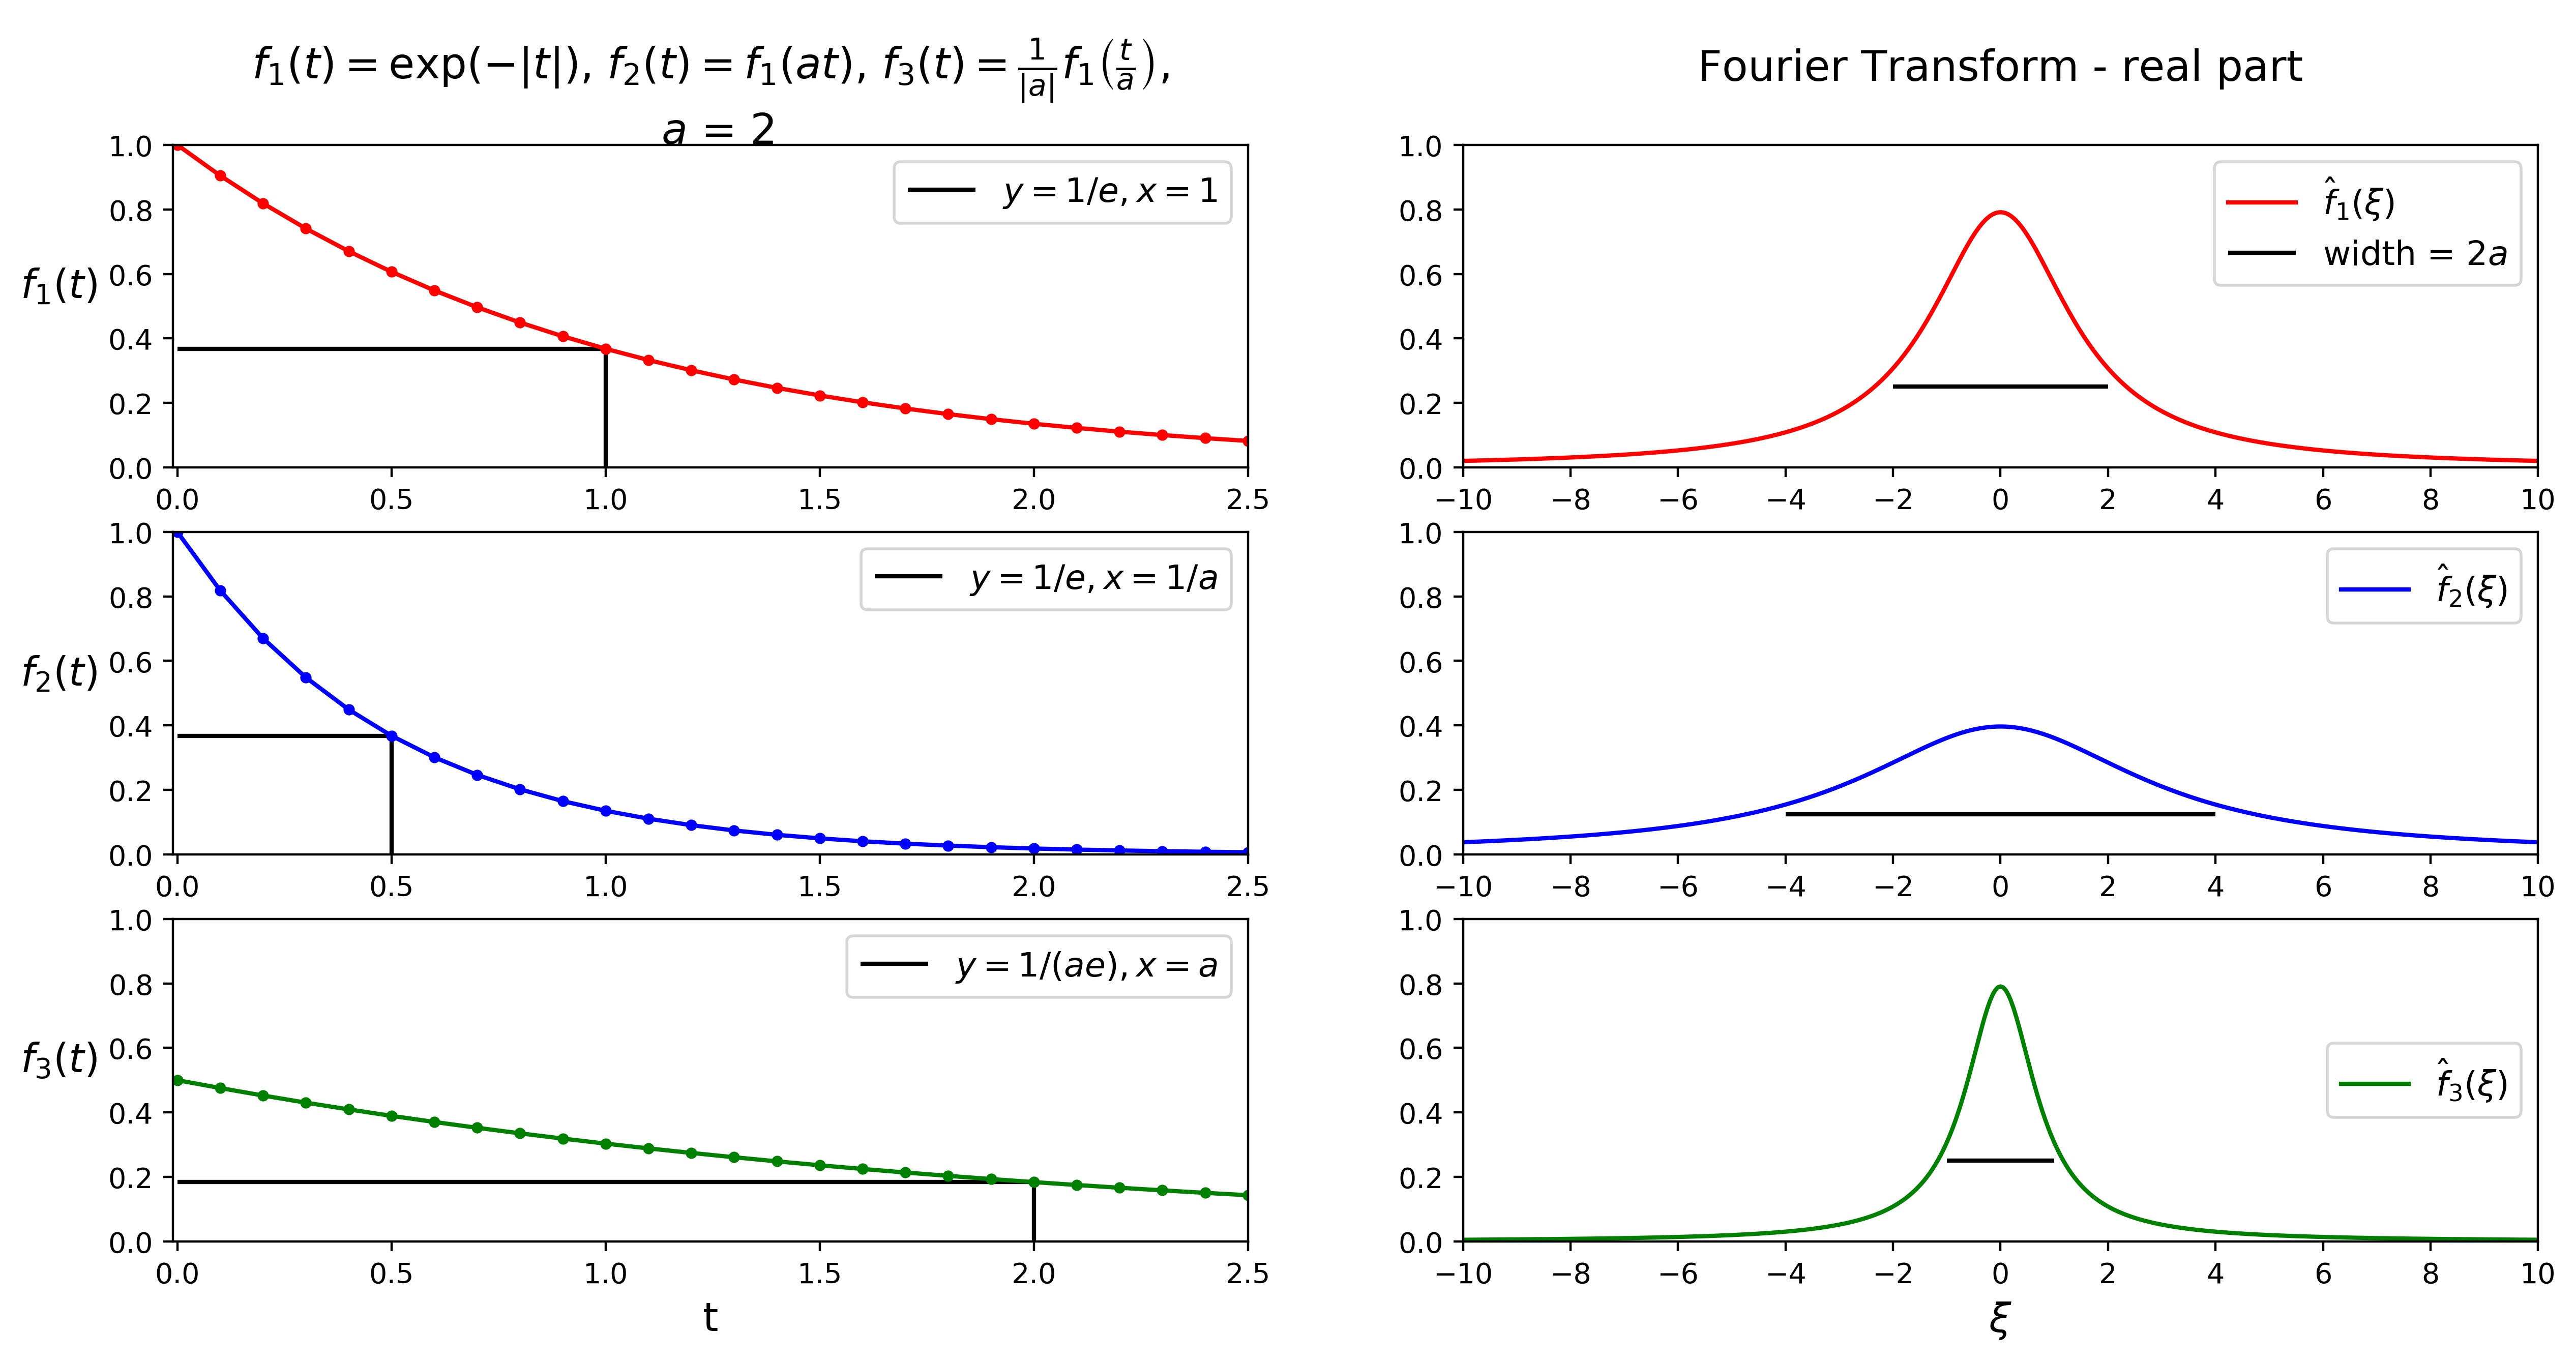
\includegraphics{../scripts/exercicio3/exp_scaling.jpg}}	
	\end{center}
	\vspace{-2mm}	% acrescentar o espaçamento vertical apropriado entre a borda inferior da figura e a legenda ou a fonte quando não há legenda (o valor pode ser negativo para subir)
	%\legenda{Figura 1.1: Dez sinais e seus respectivos histogramas para  asérie com $N$ = 64 do grupo noise.}	% legenda - para deixar sem legenda usar comando \legenda{} (nunca deve-se comentar o comando \legenda)
	\label{ex1_fig1}
	%\FONTE{}	% fonte consultada (elemento obrigatório, mesmo que seja produção do próprio autor)
\end{figure}

A Figura 3.1 explora a função $f_{1}(t)=e^{-|t|}$ (topo à esquerda), cuja transformada é $\hat{f}(\xi) = 2/(\xi^{2} + 1)$ (topo à direita). Também na esquerda, gráficos da função original e de suas consequentes funções noutras escalas: $f_{2}(t) = f_{1}(at)$ (meio) e $f_{3}(t) = f_{1}(t/a)/|a|$ (abaixo). A escolha de $a=2$ foi feita. Os valores de $x$ quando $y=1/ e$ (ou $y=1/(|a|e)$ no caso de $f_{3}(t)$) ilustram o efeito da escala nas funções $f_{2}(t)$ e $f_{3}(t)$ com relação à função original $f_{1}(t)$. À direita, suas respectivas transformadas de Fourier também exibem o efeito da escala, porém no domínio da frequência, com a largura à meia altura da transformada sinalizada em linha preta. O gráfico de $\hat{f}_{2}(\xi)$ (meio à direita) tem largura à meia altura que é o dobro de $\hat{f}_{1}(\xi)$, enquanto que sua altura é a metade deste. A largura à meia altura de $\hat{f}_{3}(\xi)$ (abaixo à direita) é metade da de $\hat{f}_{1}(\xi)$, enquanto que sua altura é igual à deste. Ou seja, em comparação a $\hat{f}_{1}(\xi)$, $\hat{f}_{2}(\xi)$ foi achatado e $\hat{f}_{3}(\xi)$ foi comprimido. 

Essa análise foi realizada com a rotina \texttt{numpy.fft.hfft}, que computa a transformada de um input com simetria Hermitiana, ou seja, gera um espectro real. As diferentes alturas da transformada resultante não foi quantitativamente analisada pois depende da normalização do algoritmo implementado. O output desta rotina não é normalizada, portanto foi aplicada a normalização $1/\sqrt{n}$. Deste modo, a análise relativa (alturas de $\hat{f}_{2}(\xi)$  e $\hat{f}_{3}(\xi)$ com relação à altura de $\hat{f}_{1}(\xi)$) permite verificação das propriedades sob estudo sem perda de generalidade.

% EXEMPLO PARA ADICIONAR FIGURA
\begin{figure}[ht!]
	\legenda{Figura 3.2: Exemplo de \textit{time scaling} e \textit{frequency scaling} sobre a função de pulso retangular com altura 4 e largura $2 \pi$.}
	\vspace{2mm}	% acrescentar o espaçamento vertical apropriado entre o título e a borda superior da figura
	\begin{center}
		\resizebox{\textwidth}{!}{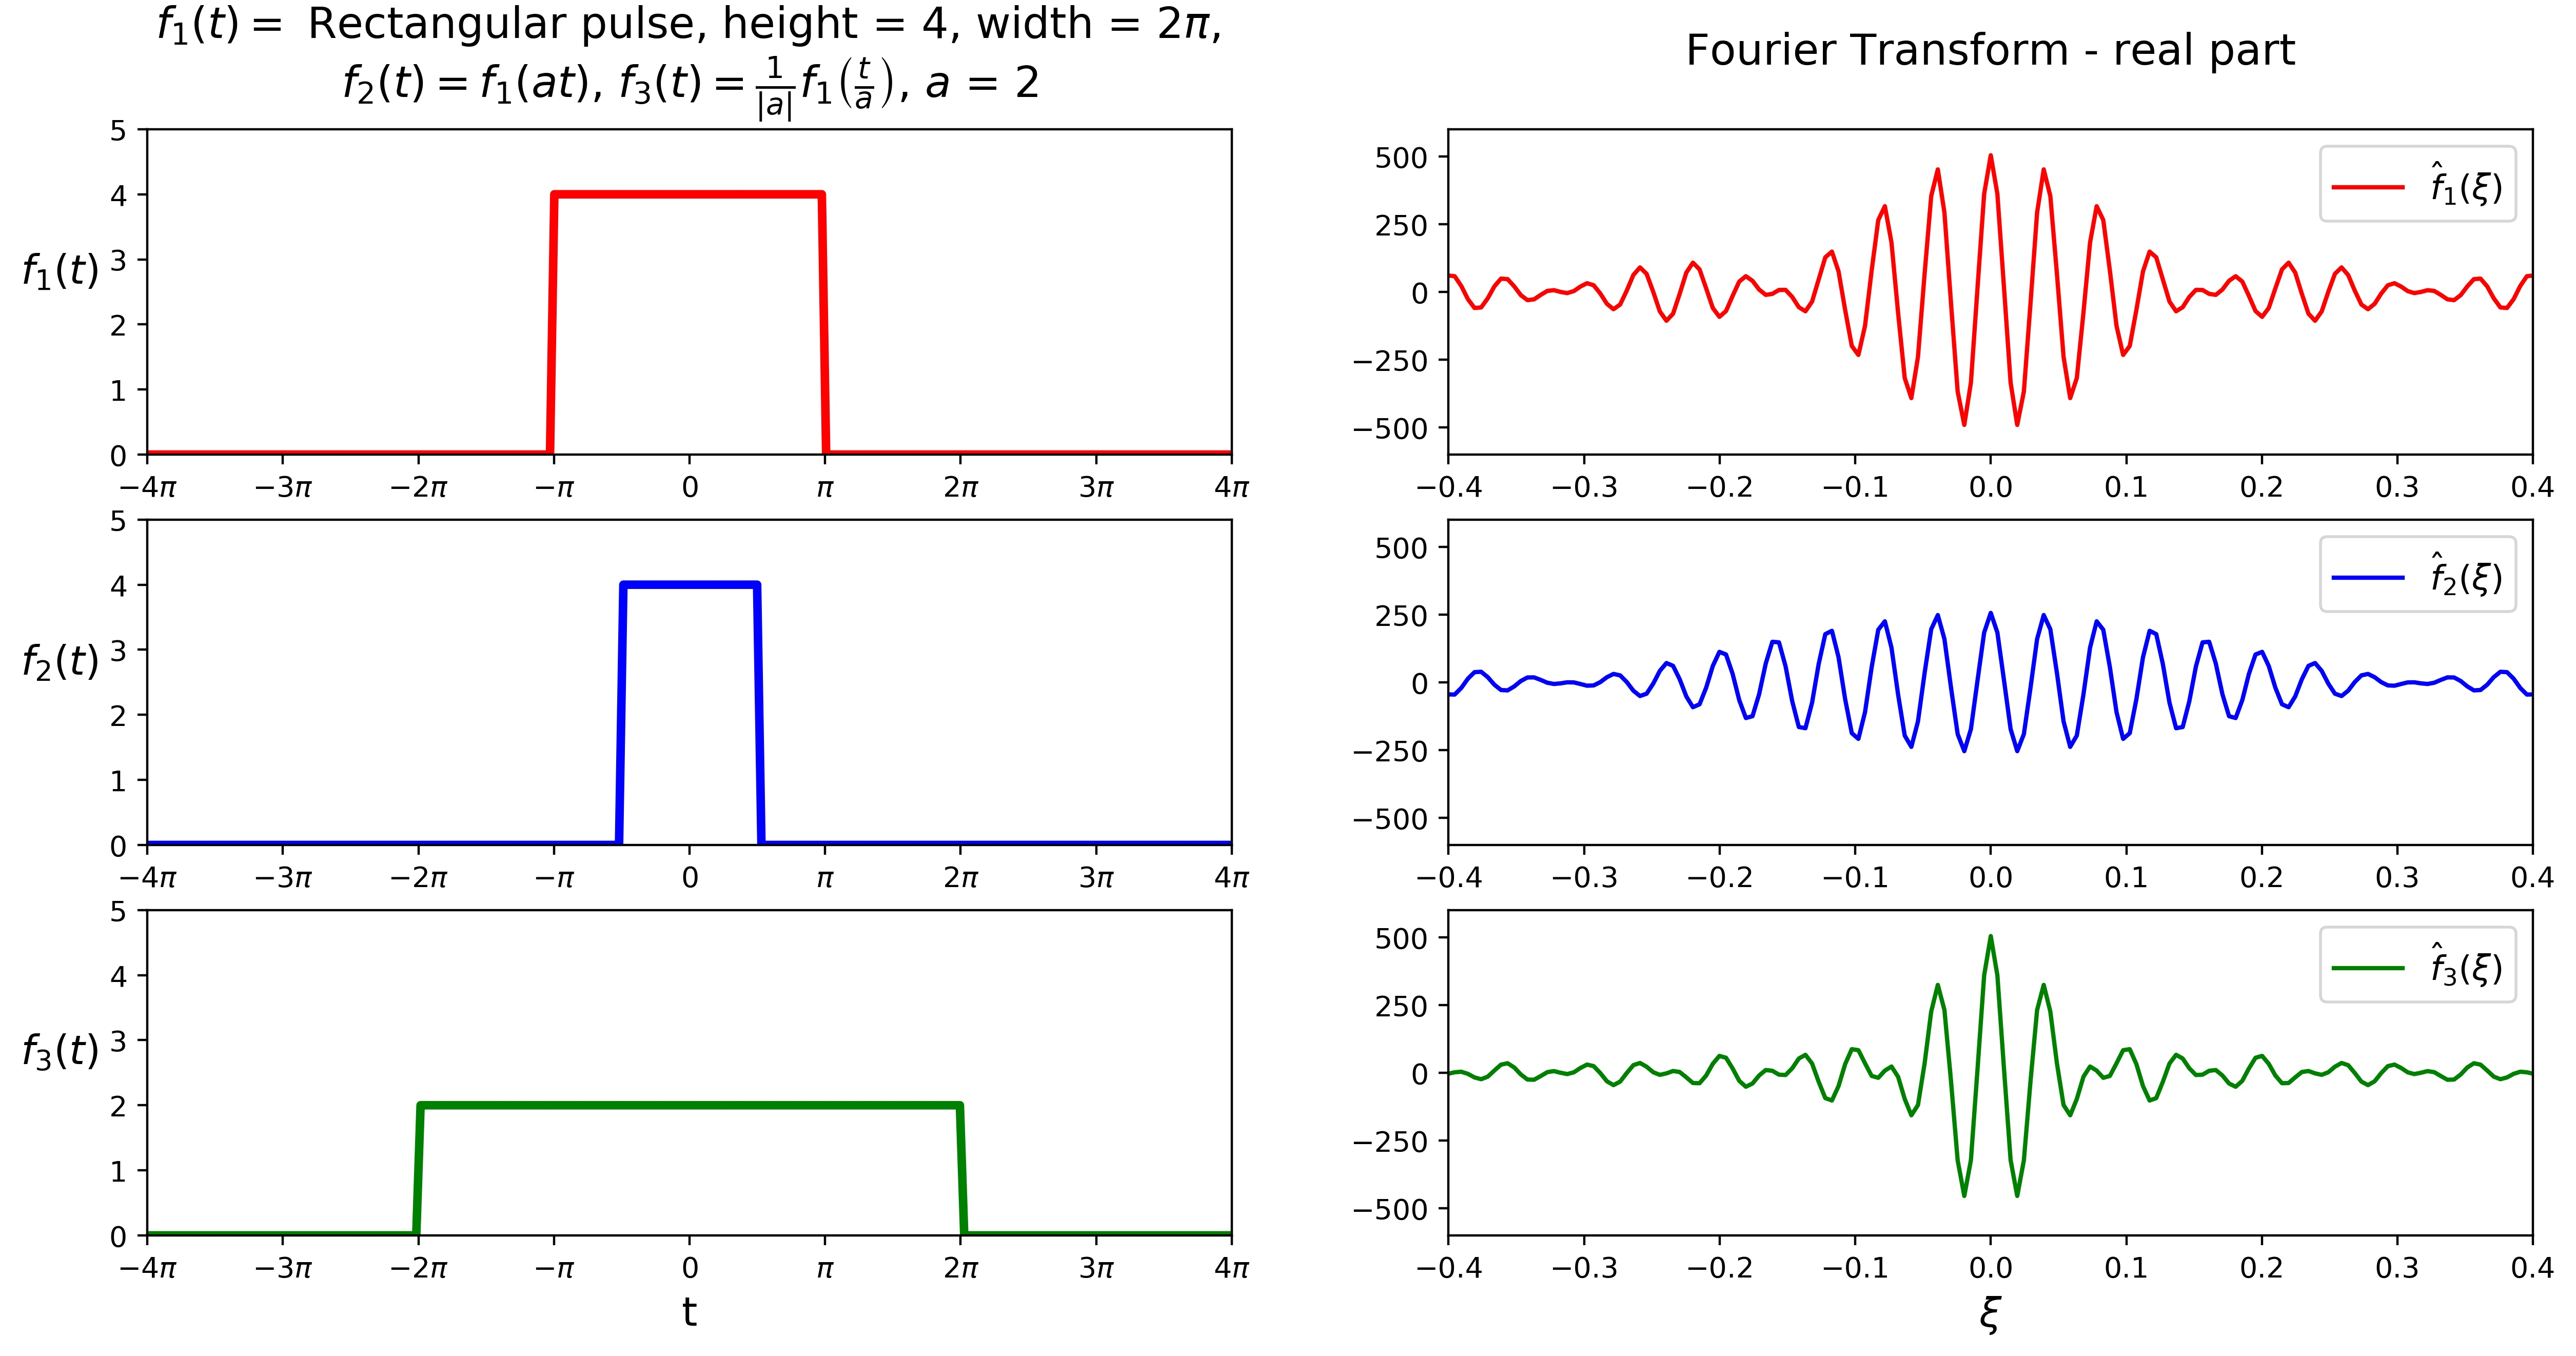
\includegraphics{../scripts/exercicio3/square_scaling.jpg}}		
	\end{center}
	\vspace{-2mm}	% acrescentar o espaçamento vertical apropriado entre a borda inferior da figura e a legenda ou a fonte quando não há legenda (o valor pode ser negativo para subir)
	%\legenda{Figura 1.1: Dez sinais e seus respectivos histogramas para  asérie com $N$ = 64 do grupo noise.}	% legenda - para deixar sem legenda usar comando \legenda{} (nunca deve-se comentar o comando \legenda)
	\label{ex1_fig1}
	%\FONTE{}	% fonte consultada (elemento obrigatório, mesmo que seja produção do próprio autor)
\end{figure}

A Figura 3.2 exemplifica as propriedades de \textit{time} e \textit{frequency scaling} a partir de uma função pulso retangular. A altura do pulso original (topo à esquerda) é igual a quatro e a largura é $2 \pi$. Os demais gráficos da esquerda são sinais sob diferentes efeitos da escala $a=2$, e na direita estão suas respectivas transformadas. Assim como na Figura 3.1, os efeitos de achatar, esticar e comprimir o sinal no domínio do tempo são evidentes: achatá-lo no tempo estica-o na frequência (\textit{time scaling}), enquanto que esticá-lo e comprimi-lo no tempo mantém sua magnitude porém achata-o na frequência (\textit{frequency scaling}).

%====================================================================== 3.2

\subsection*{3.2}
\addcontentsline{toc}{section}{\protect\numberline{} 3.2}%

A Figura a seguir ilustra as propriedades de \textit{time shifting} e \textit{frequency shifting}:

\begin{align*}
f(t - t_{0}) &\Leftrightarrow \hat{f}(\xi)e^{2 \pi \imath \xi t_{0}} \tag*{\textit{time shifting}} \\
f(t)e^{2 \pi \imath \xi_{0} t} &\Leftrightarrow \hat{f}(\xi - \xi_{0})  \tag*{\textit{frequency shifting}} 
\end{align*}

% EXEMPLO PARA ADICIONAR FIGURA
\begin{figure}[h!]
	\legenda{Figura 3.3: Exemplo de \textit{time shifting} e \textit{frequency shifting} sobre a função $\cos(2 \pi t/10)$.}
	\vspace{2mm}	% acrescentar o espaçamento vertical apropriado entre o título e a borda superior da figura
	\begin{center}
		\resizebox{\textwidth}{!}{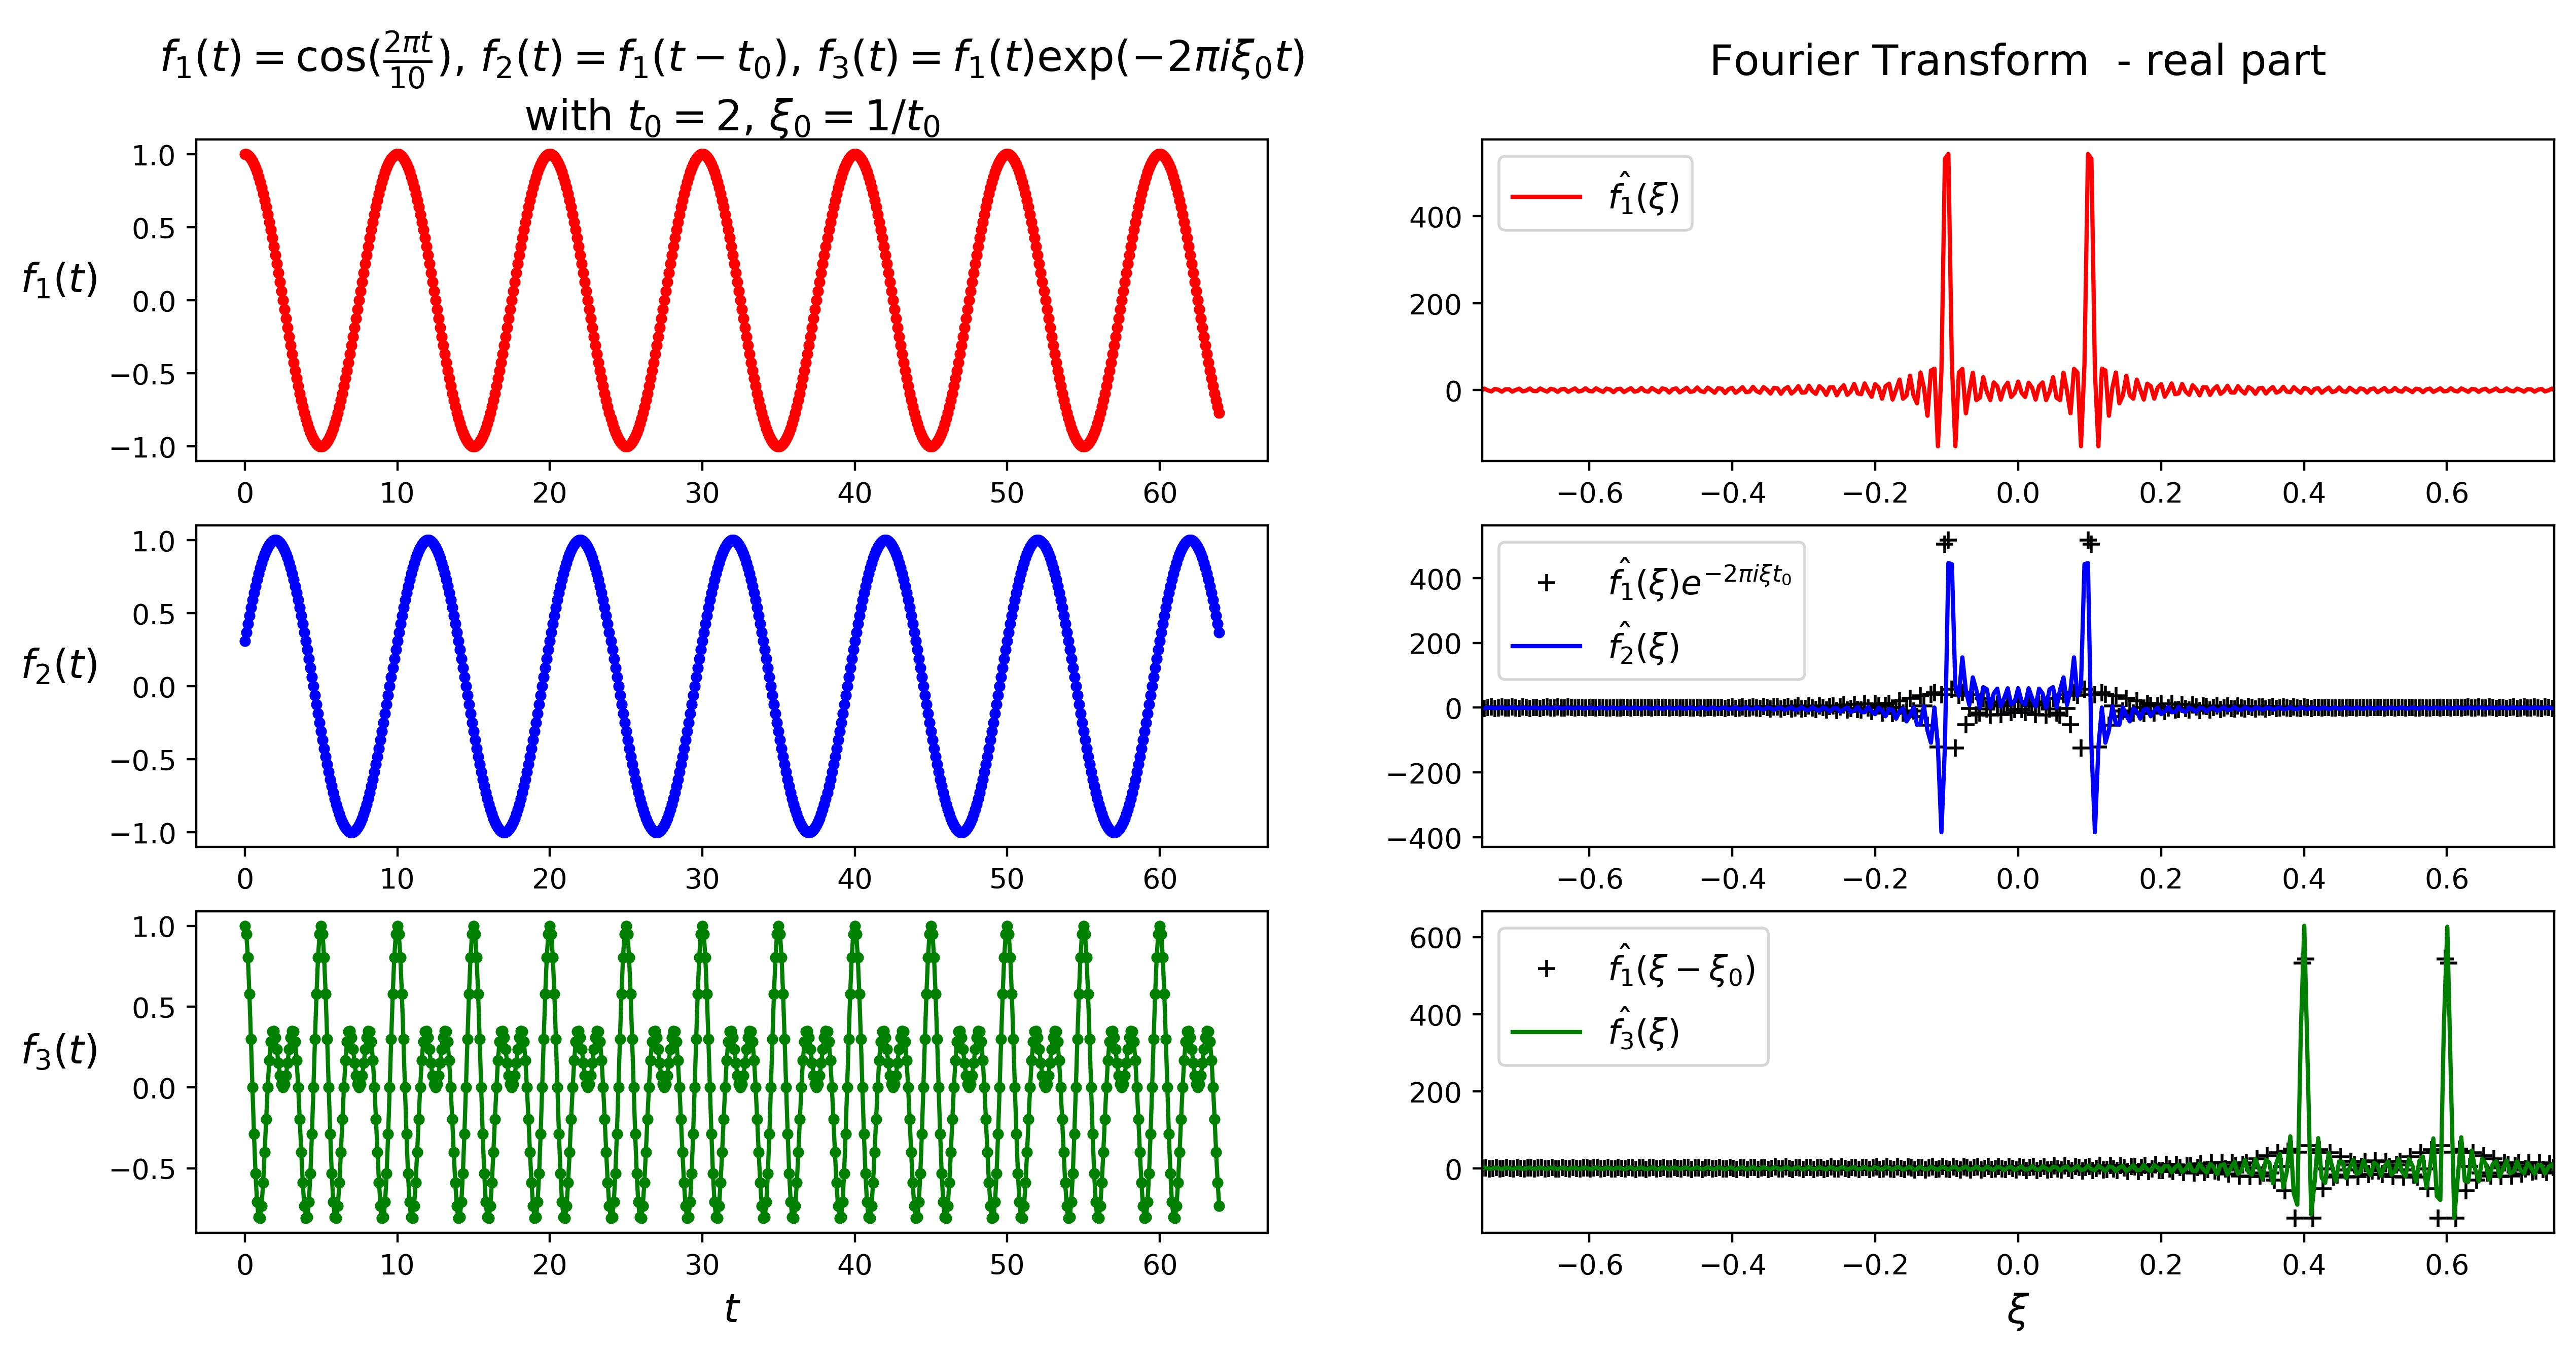
\includegraphics{../scripts/exercicio3/time_shifting.jpg}}		
	\end{center}
	\vspace{-2mm}	% acrescentar o espaçamento vertical apropriado entre a borda inferior da figura e a legenda ou a fonte quando não há legenda (o valor pode ser negativo para subir)
	%\legenda{Figura 1.1: Dez sinais e seus respectivos histogramas para  asérie com $N$ = 64 do grupo noise.}	% legenda - para deixar sem legenda usar comando \legenda{} (nunca deve-se comentar o comando \legenda)
	\label{ex1_fig1}
	%\FONTE{}	% fonte consultada (elemento obrigatório, mesmo que seja produção do próprio autor)
\end{figure}

No topo à esquerda a função $\cos(2 \pi t/10)$ é graficada com sua transformada de Fourier à direita. Também à esquerda estão a função $f_{2}(t)$ (meio) e $f_{3}(t)$ (abaixo) que representam as propriedades de \textit{time shifting} e \textit{frequency shifting}, respectivamente. Suas trasformadas de Fourier à direita ($\hat{f}_{2}(\xi)$ no meio e $\hat{f}_{3}(\xi)$ abaixo) são graficadas junto com pontos de ajuste da função $\hat{f}_{1}(\xi)$ com sinais de `+' na cor preta. Os pontos resultantes estão sobrepostos às transformadas das funções $f_{2}(t)$ e $f_{3}(t)$, evidenciando as propriedades de \textit{time} e \textit{frequency shifting}.








